\apendice{Plan de Proyecto Software}

\section{Introducción}

%Ojo \footnote{Los anexos deben de tener su propia bibliografía, eso es tan fácil como utilizar referencias igual que en la memoria \cite{bortolot2005}}

\section{Planificación temporal}

\begin{figure}[ht]
    \centering
    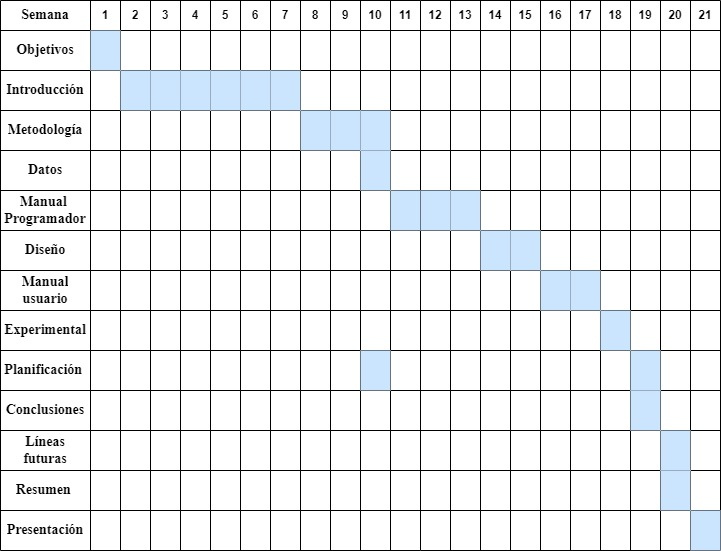
\includegraphics[width=0.85\textwidth]{img/planificacionTFG.jpg}
    \caption{Planificación temporal}
    \label{fig:plan-temporal}
 \end{figure}

\subsection{Planificación económica}

\begin{table}[ht]
	\centering
	\begin{tabularx}{\linewidth}{ p{0.6\columnwidth} p{0.71\columnwidth} }
		\toprule
		\textbf{Materiales}    & \textbf{Precio}\\
		\toprule
		\textbf{Placa Arduino Uno}              & precio \\
		\textbf{MPU-6050}                & precio \\
        \textbf{Módulo HC-05}              & precio    \\
        \textbf{Módulo ESP8266}              & precio    \\
		\bottomrule
	\end{tabularx}
	\caption{Planificación económica}
\end{table}

\subsection{Viabilidad legal}

